%\documentclass[preprint,twocolunn]{aastex}
%\documentclass[apj, twocolumn, preprint]{aastex}
\documentclass[apj]{emulateapj}
\newcommand{\nuobs}{\nu_o}
\newcommand{\nuemit}{\nu_e}
\newcommand{\lambdaobs}{\lambda_o}
\newcommand{\lambdaemit}{\lambda_e}
\usepackage{graphicx}

\graphicspath{{/Users/amandanewmark/repositories/galaxy_dark_matter/lumprofplots/clumps/}{/Users/amandanewmark/repositories/galaxy_dark_matter/lumprofplots/distribution/}{/Users/amandanewmark/Desktop/}{/Users/amandanewmark/repositories/galaxy_dark_matter/reports/}}

%\shorttitle{Understanding Mass Assembly of Luminous Red Galaxies in HSC}
%\shortauthors{Amanda Newmark}

\begin{document}

 \title{Understanding Mass Assembly of Luminous Red Galaxies in HSC}
 \author{Amanda Newmark and Elinor Medezinski}
 \date{August 2016}

\begin{abstract}
The slope of the stellar envelopes of galaxies are thought to reflect the mass assembly history and is connected to their underlying Dark Matter Halos. In this study, we use the Hyper Suprime-Cam (HSC) Survey to probe the stellar envelopes of Luminous Red Galaxies (LRGs) to better understand this relationship. We make use of the HSC multi-aperture magnitudes measured for BOSS/LOWZ galaxies to construct luminosity density profiles. We find the slope of the stellar envelope, $\alpha_{stars}$, by fitting the stacked luminosity density profile at large comoving distances, 22 kpc $< R <$ 61 kpc. Finding consistent slopes of younger and older galaxies, we conclude that there is no correlation between star formation epoch and mass assembly history for those massive, red, early-type galaxies.
\end{abstract}

\section{Introduction}
Galaxies are often studied through their luminosity profiles. Beyond the bright central bulge lies a fainter stellar structure called the stellar halo, which is often measured directly through star counts (\cite{DSouza:2014}). The luminosity in the outer component of the stellar halo measures the amount of stellar light accreted in the galaxy through mergers with satellites. Through studying the varying surface brightness of the stellar envelope, we see direct evidence of the mass accretion history of the galaxy. 

We are interested in what governs the buildup of the stellar envelope. As galaxies merge with satellites, they grow from the inside out, forming larger and larger stellar envelopes. Visible aspects of the stellar envelope are affected (i.e. the distribution of stars). However, the dark matter is also tidally disrupted.

Previous observational experiments have studied different aspects of the stellar envelope. For example, using the Galaxy and Mass Assembly (GAMA) survey, \cite{Bauer:2013} investigates Star Formation History (SFH) as a function of stellar mass. They focus on mass accumulated in-situ, rather than through mergers.  However, this study does not specifically probe the stellar envelope.

\cite{Iodice:2016} used the Fornax Deep Survey, a multi-imaging survey, to probe the core of the Fornax cluster, NGC 1399. This study revealed that the core is characterized by a diffuse envelope surrounding NCH 1399. Examining this galaxy hints that the stellar envelope is made of stripped stars from neighbor galaxy, NGC 1387, and therefore is undergoing a major merging event. This was only accomplished for a single galaxy, not a sample of galaxies.


\begin{figure}[htb!]
\centering
\includegraphics[width=.45\textwidth]{Pillepich_1}
\caption{\scriptsize{This figure shows 2D simulations of mass assembly of two different types of galaxies, an elliptical (upper row) and a disk (lower row). The third column shows the slope of the stellar envelopes, $\alpha_{stars}$. (\cite{Pillepich:2014})}}
\label{fig:meshaaa}
\end{figure}

From previous simulations, the slope of the outer stellar envelope ($\alpha_{stars}$) are thought to be direct evidence of the evolution of Dark Matter Haloes and their mass assembly histories (\cite{Pillepich:2014}). In Figure \ref{fig:meshaaa}, Pillepich, using the Illustris Simulations, demonstrates the mass assembly of elliptical and disk galaxies. We see that the environment surrounding elliptical galaxies are much lumpier, showing how it is accreting nearby galaxies. Pillepich then fits the outer averaged density profiles to a single power law, setting her limits from the half-light radius, $R_{1/2}$, to the virial radius, $R_{vir}$ (\cite{Pillepich:2014}). The half-light radius is considered the innermost boundary of the stellar envelope, while the virial radius is thought to mark the outskirts.

We are interested in finding a correlation between a Luminous Red Galaxy's (LRG) mass assembly history and the Dark Matter Halo. In our study, we plan to probe the stellar envelopes of LRGs to assess the codependence of the Dark Matter Halo and Mass assembly. We focus on LRGs because they are a well defined, homogeneous population. LRGs are all red and dead galaxies: higher mass ellipticals with little to no star formation.

\section{Data}

\begin{deluxetable}{ccc}
\tabletypesize{\footnotesize}
\tablecaption{\scriptsize{Diameters assume a pixel scale of 0.168 ($arc/sec$)} \label{table:1}}
\tablehead{Aperture number & Radius (pixels) & Diameter (arcseconds)}
\startdata
aperture00& 3.0 & 1.01\\
aperture01 & 4.5 &1.51  \\
aperture01 &6.0 &2.02\\
aperture03 &9.0 &3.02\\
aperture04 &12.0 &4.93 \\
aperture05 &17.0 &5.71 \\
aperture06 &25.0 &8.40 \\
aperture07 &35.0 &11.7\\
aperture08 &50.0 &16.8\\
aperture09 &70.0 &23.5\\
\enddata
\end{deluxetable}

There is a coevolution of dark and visible matter throughout the formation of LRGs. By fitting the slopes of the stacked luminosity density profiles, we hope to connect the stellar envelope to the Dark Matter Halo. We will use the Hyper Suprime-Cam (HSC) Survey to obtain the luminosity density profiles of our sample galaxies.

\begin{figure}
\centering
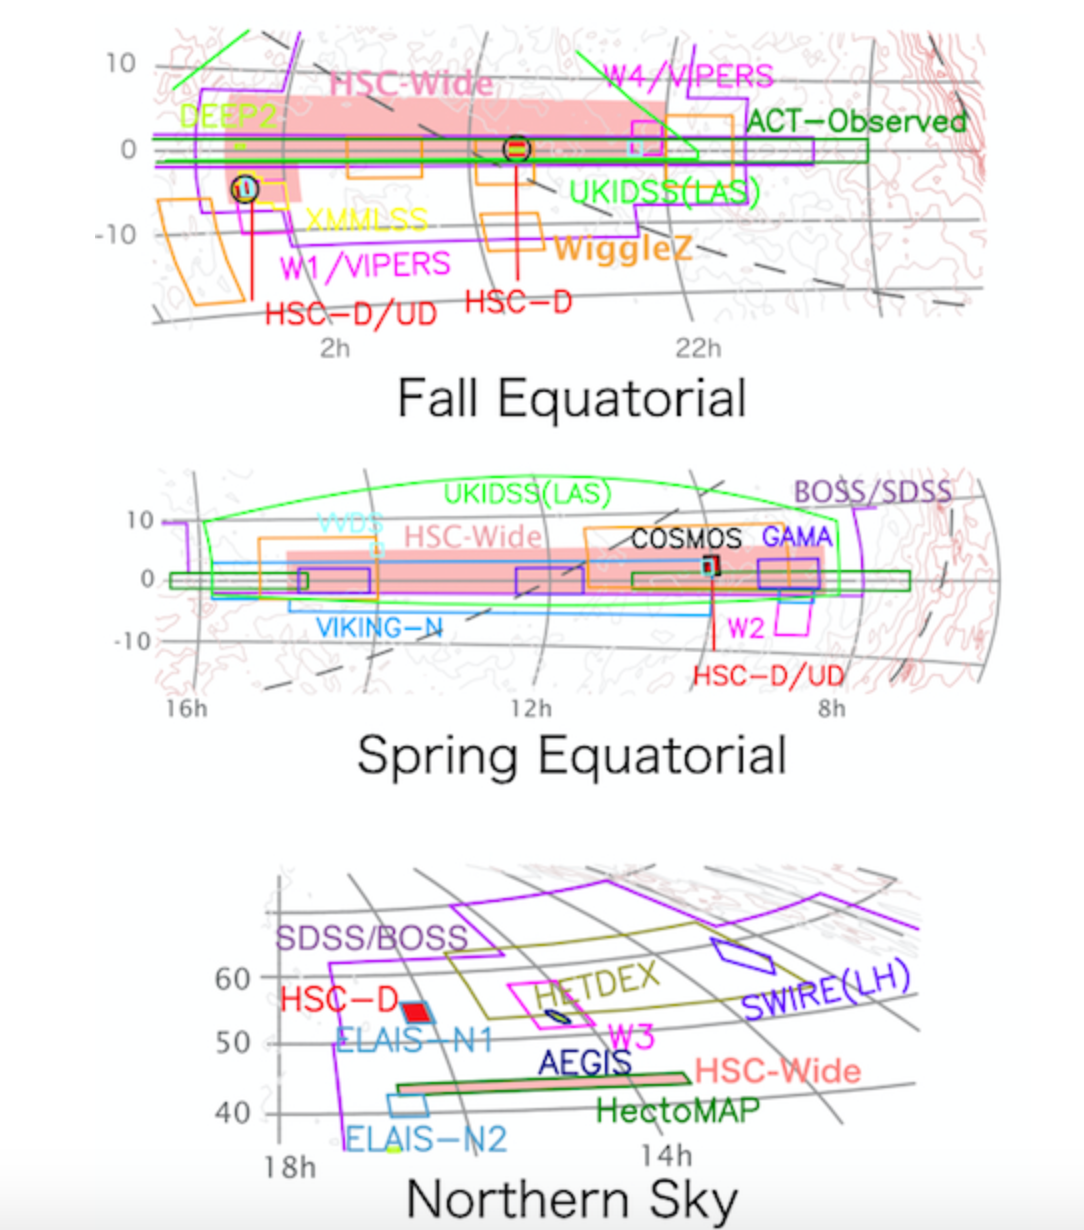
\includegraphics[width=.4\textwidth]{HSC_regions}
\caption{HSC survey fields, consisting of the Fall Equatorial, Spring Equatorial, and Northern Sky regions.}
\label{fig:hsc-reg}
\end{figure}

HSC is a multi-band imaging survey, containing Wide, Deep, and Ultra Deep layer fields. We are using one of six Wide layer fields, which covers 1400 deg$^2$ in the sky in the \textit{g, r, i, z,} and \textit{y} bands. The Wide field covers the Fall equatorial, Spring equatorial, and Northern sky regions shown in Figure \ref{fig:hsc-reg}. This field surveys galaxies at redshifts up to z$\sim$1, and will measure weak gravitational lensing (which will be used in the next step of this study),

For our experiment, we use the \textit{i} band because it can probe the faintest magnitudes. In order to get the luminosity profiles of the galaxies, we use the magnitudes for the LOWZ/BOSS LRGs at ten spherical apertures. The apertures are listed in Table \ref{table:1}.

As previously stated, there have been other observational studies that use stellar profiles as a probe of mass assembly. However, HSC goes to very low surface brightness for more galaxies and can probe the envelope better. We can study the dimmest parts of the stellar envelope that other tools cannot detect. Therefore, we believe it is the best tool for this experiment.

The Sloan Digital Sky Survey (SDSS), a multi-imaging survey, has already imaged over 35\% of the sky. It selects the LRG sample on a basis of color and magnitude, which holds up to z=0.38 (\cite{Eisenstein:2001}.) The Baryon Oscillation Spectroscopic Survey (BOSS) targets two different populations of galaxies: the "Constant Stellar Mass" (CMASS), or the low-redshift sample (LOWZ) (\cite{Cuesta:2015}). We use the BOSS/LOWZ galaxies because they cover redshifts between 0.15 and 0.43, within the SDSS LRG sample redshift uperlimit. Using the Right Ascension $\alpha$ and Declination $\delta$ coordinates from the SDSS query, we match this with the HSC catalogue to identify the corresponding LRGs. Our final catalogue contains 1561 LRGs with accurate results.

\section{Methodology}

Our catalogue provides the apparent magnitudes taken at ten different apertures, shown in Table \ref{table:1}. First, we have to get the absolute magnitudes for each aperture. We wish to know the absolute magnitude \textit{M} from its apparent magnitude \textit{m}, and therefore follow this equation from the article "The K Correction" \cite{Hogg:2002}
\begin{equation}
\small{
m_R=M _Q+ DM + K_{QR} \;\;\;,
}
\end{equation}

where $R$ is the observed bandpass and $Q$ is the emitted bandpass. The distance modulus (DM) is 
\begin{equation}
\small{
DM = 5\,\log_{10}\left[\frac{D_L}{10~\mathrm{pc}}\right] \;\;\;.
}
\end{equation}

Since our sample of galaxies are all observed at different redshifts, the \textit{K}Correct parameter corrects this discrepancy
\begin{equation}
\scriptsize{
K_{QR} = -2.5\,\log_{10}\left[[1+z]\,
  \frac{\displaystyle\int\frac{\mathrm{d}\nuobs}{\nuobs}\,f_{\nu}(\nuobs)\,R(\nuobs)\,
          \int\frac{\mathrm{d}\nuemit}{\nuemit}\,g^Q_{\nu}(\nuemit)\,Q(\nuemit)}
       {\displaystyle
          \int\frac{\mathrm{d}\nuobs}{\nuobs}\,g^R_{\nu}(\nuobs)\,R(\nuobs)\,
          \int\frac{\mathrm{d}\nuemit}{\nuemit}\,
            f_{\nu}\!\left(\frac{\nuemit}{1+z}\right)\,Q(\nuemit)}\right] \;\;\;.
            }
\end{equation}

Once we obtain all of the absolute magnitudes, we convert to luminosity using
\begin{equation}
\small{
L_Q=10^{-0.4(\textit{M}-\textit{M}_{\odot})} \;\;\;,
}
\end{equation}

where $\textit{M}_{\odot}$ is the magnitude of the Sun within filter $Q$. 

Finally, in order to obtain our luminosity densities, we must convert our apertures to comoving distance ($R$). Our galaxies are not all located at the same distance, and the comoving distance, given in kiloparsecs (kpc), is the proper distance for each aperture, after factoring out the different redshifts. Finally, luminosity density $\rho$ is given as
\begin{equation}
\small{
\rho_L=L/(4\pi R^2)
}
\end{equation}

\section{Results}
\subsection{Testing Photometric Issues}
In order to certify the validity of our results, it is essential that we test the photometric contamination caused by fainter galaxies that are not properly resolved, or \textit{deblended}. Such galaxies can contaminate the apparent magnitude of the galaxy, most prominently at the outer stellar halo of the galaxy.

\begin{deluxetable}{c}
\tabletypesize{\footnotesize}
\tablecaption{\scriptsize{Flags from our LOWZ/BOSS catalogue}  \label{table:2}}
\tablehead{Flags}
\startdata
Saturated Center\\
Cosmic Ray \\
Bad Pixels \\
Suspect \\
Clipped\\
Edge\\
Interpolated Centers \\
\enddata
\end{deluxetable}

The HSC pipeline flags specific galaxies which are contaminated. The types of flags are listed in Table \ref{table:2}.  After disregarding these galaxies, we have 1075 remaining LRGs.

The Bright Objects flag is a conservative flag, meaning there is a nearby bright star that overlaps with the stellar envelope of a galaxy. This would make that galaxy appear brighter. Since galaxies flagged as Bright Objects make up about a third of our remaining sample of galaxies (337), we have to determine whether or not these should be disregarded. 

\begin{figure*}[htp!]
\centering
\begin{minipage}[b]{0.45\linewidth}
  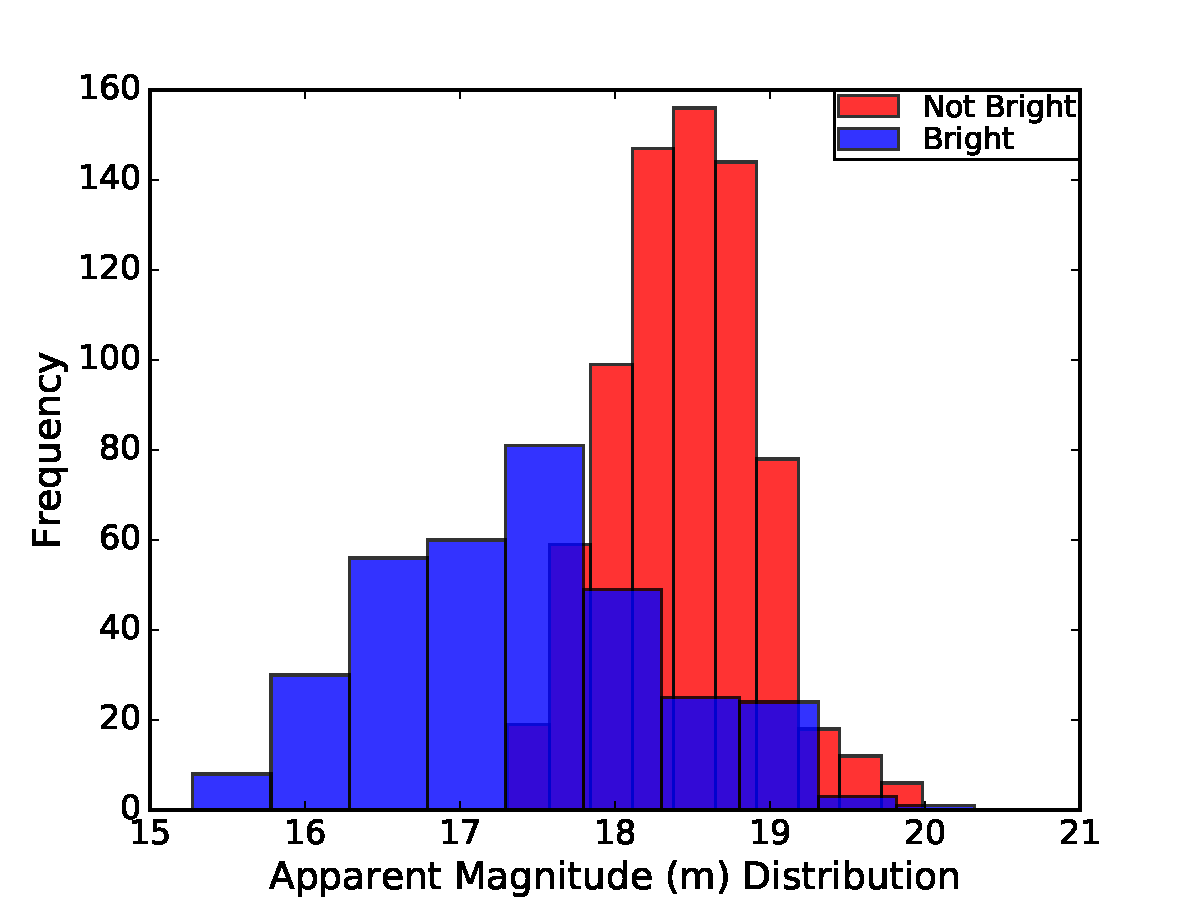
\includegraphics[width=\textwidth]{3meanuplimmagdist.pdf}
  \caption{\scriptsize{Apparent Magnitude (m) Distributions for Not Bright Objects (red) and Bright Objects (blue).}}
  \label{fig:sfig11}
\end{minipage}
\quad
\begin{minipage}[b]{0.45\linewidth}
 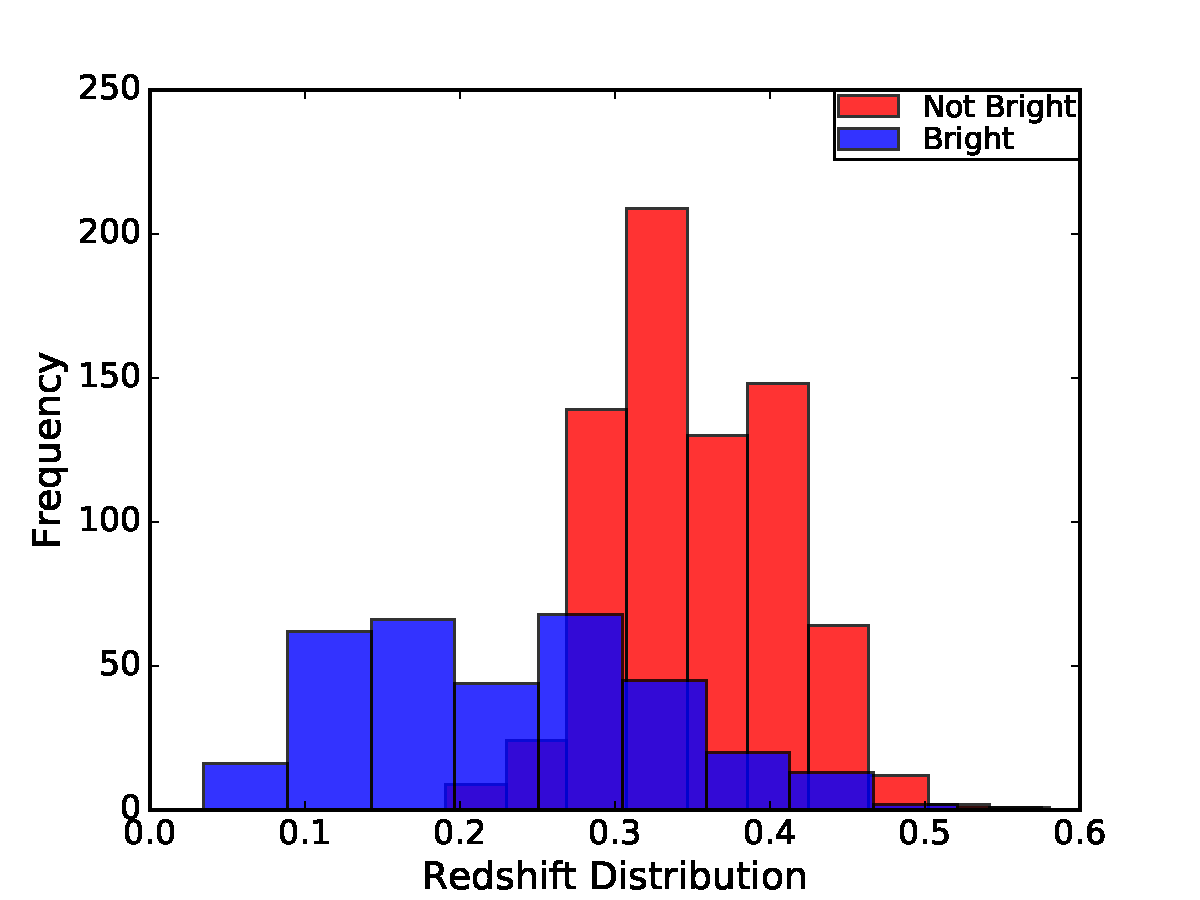
\includegraphics[width=\textwidth]{3meanuplimzdist.pdf}
  \caption{\scriptsize{Redshift (Z) Distributions for Not Bright Objects (red) and Bright Objects (blue).}}
  \label{fig:sfig12}
\end{minipage}
\end{figure*}

To determine whether bright object centers saturate our luminosity profiles, the LRGs are separated into two populations, one where the Bright Object flag is \textbf{True} and one where the Bright Object flag is \textbf{False}. Since we first want to confirm that these galaxies are all from the same population, in Figure \ref{fig:sfig11} and \ref{fig:sfig12}, we construct the distributions of the redshifts and apparent apparent magnitudes for flagged (blue) and not flagged (red) galaxies. 

The apparent magnitudes and redshifts for the flagged galaxies aren't normally distributed like the non-flagged galaxies. While the blue bars trail off at m=17, we also notice that they trail off at z=0.2. Since these galaxies were at a lower redshift, they would have overall smaller apertures in kpc, resulting in lower surface brightness. To correct this, we set a lower limit of 0.2 to our redshift distribution.  After implementing this cut, 191 galaxies flagged as Bright Objects remain.

\begin{figure}[h]
\centering
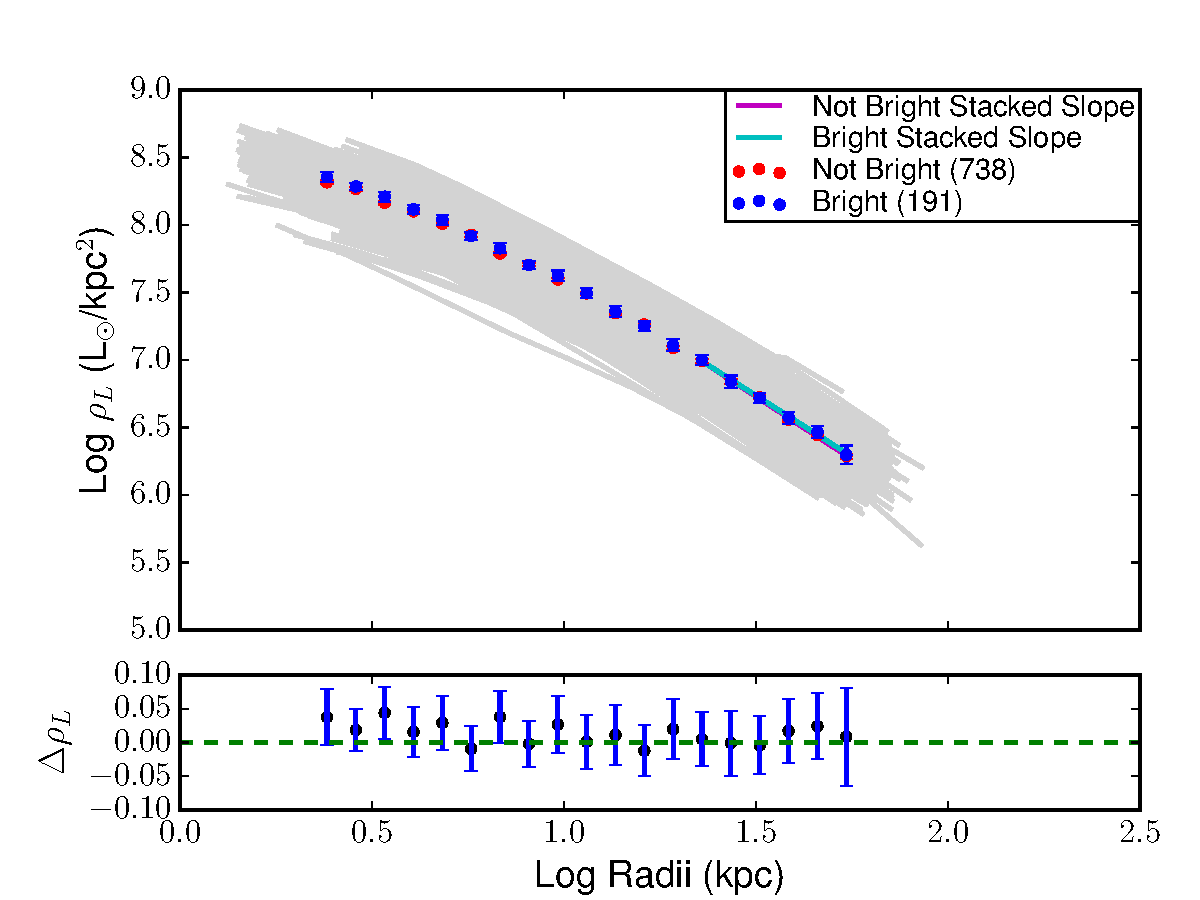
\includegraphics[width=.5\textwidth]{3+meanuplimTF.pdf}
\caption{Top graph: The luminosity profiles of all individual galaxies are represented by the gray lines. The stacked luminosity profiles of Bright galaxies (blue points) and not bright galaxies (red points) overlay the individual profiles. The lines of best fit are represented by the cyan line (Bright Stacked Slope) and magenta line (Not Bright Stacked Slope). Bottom graph: The difference between the stacked Bright and Not Bright luminosity densities at each radial bin.}
\label{fig:mesh1}
\end{figure}

Figure \ref{fig:mesh1} shows stacked luminosity profile for each flagged (blue points) and non-flagged populations (red points). In the background, I plot the luminosity profiles of the individual galaxies (gray curves).  In order to homogenize our results, so they are all fit to the same physical boundary, we set an inner boundary of $3R_{1/2}$ and an outer boundary of exactly $6R_{1/2}$ to both individual luminosity profiles and stacked profiles. 

Typically, the half light radius ($R_{1/2}$) denotes the inner boundary of the stellar halo. However, since HSC can probe to very low surface brightness, we wanted to use this tool to our advantage and only look at the outermost regions of the stellar halo. Also, in \cite{Pillepich:2014}, the outer boundary was marked by the virial radius ($R_{vir}$). Since we found that $R_{vir}$ for our galaxies extended beyond our largest measured aperture, we arbitrarily choose $6R_{1/2}$.  By implementing this outer limit, we can safely use photometry of these bright sources.

Interestingly, the slopes in Figure \ref{fig:mesh1} of the Stacked Bright Objects is -1.807  $\pm$  0.155 and that of the Stacked Not Bright Objects is -1.861  $\pm$  0.049. Therefore, the galaxies flagged as bright objects are in agreement with those not flagged. Therefore, we can conclude that it is not necessary to disregard LRGs flagged as "Bright Objects" from our sample population. 

\subsection{Star Formation History via VESPA}
Before we can assess the relationship between mass assembly and the dark matter envelope, we first need to see if there is a correlation between mass assembly and star formation history (SFH).Since LRGs are all early-type galaxies, they have undergone mergers and accumulated most of their mass at this time. Using VESPA, an algorithm that fits the spectra of all LRGs in the Sloan Digital Sky Survey's (SDSS) final data release, we match with our original catalogue to get their SFH (\cite{Tojeiro:2009}). Figure \ref{fig:meshba1} depicts the mass fractions as a function of age for one galaxy measured by VESPA.

\begin{figure}[htp!]
\centering
\begin{minipage}[b]{0.75\linewidth}
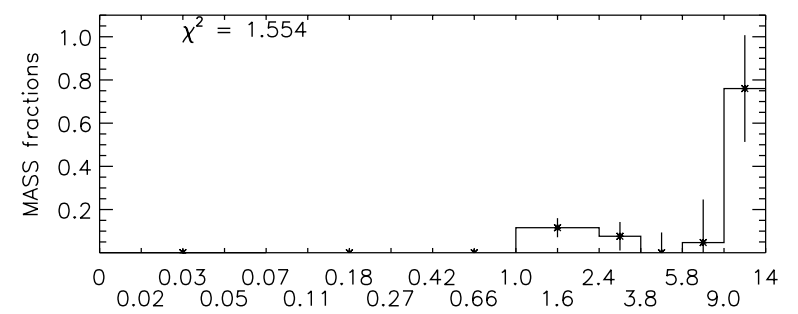
\includegraphics[width=\textwidth]{massfrac}
\caption{The mass assembly histories from \cite{Tojeiro:2009}.}
\label{fig:meshba1}
\end{minipage}
\quad
\begin{minipage}[b]{0.75\linewidth}
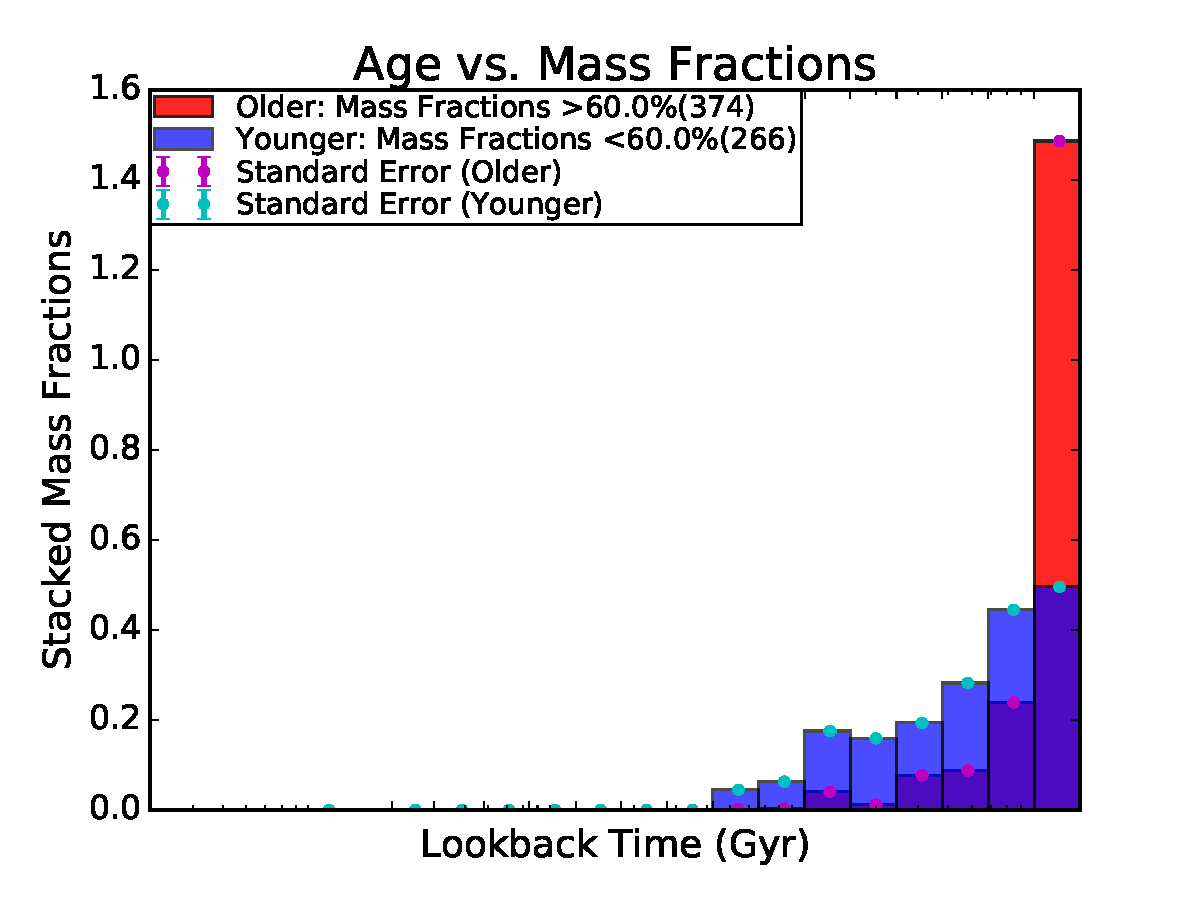
\includegraphics[width=\textwidth]{oy_agebin.pdf}
\caption{The mass factions of older galaxies (red) and younger galaxies (blue) from our catalogue.}
\label{fig:meshba2}
\end{minipage}
\end{figure}


\begin{figure}[htb!]
\centering
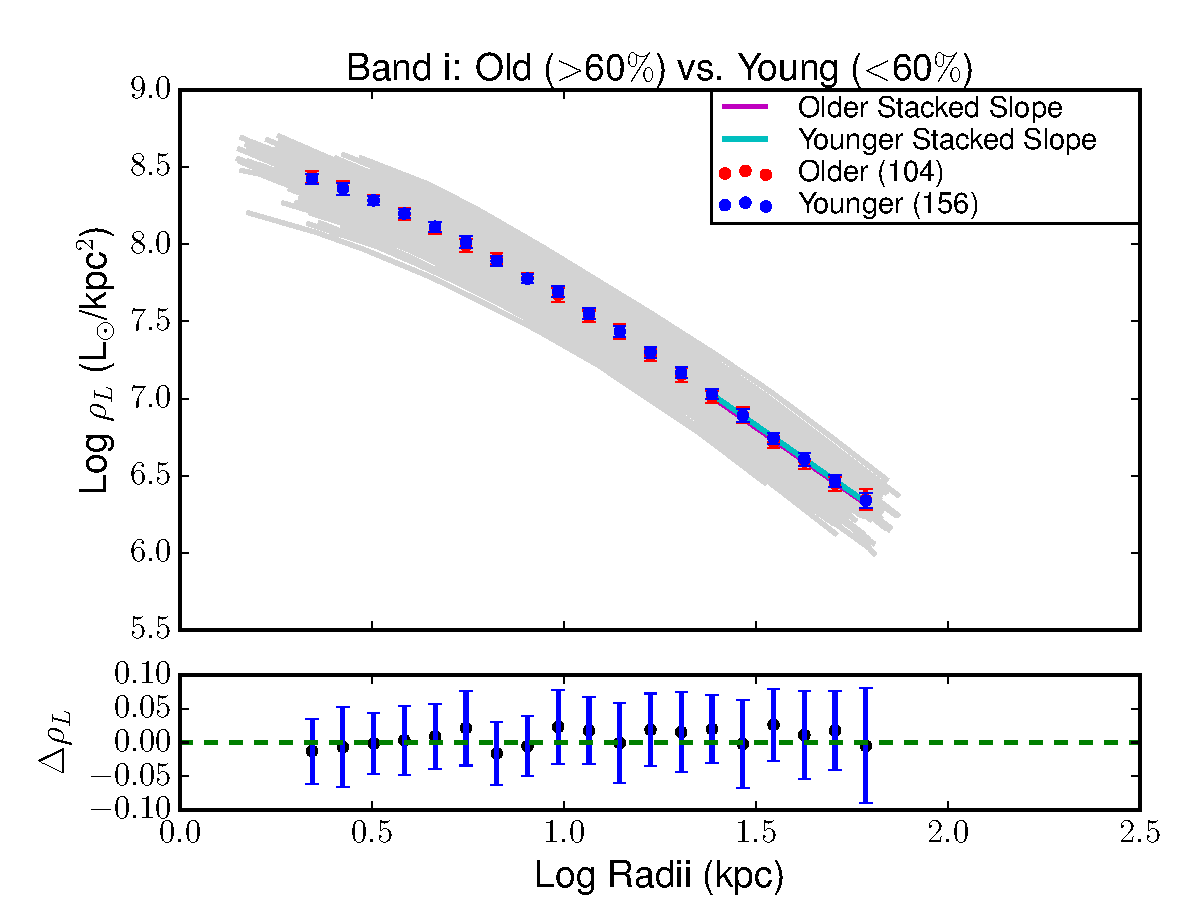
\includegraphics[width=.5\textwidth]{3+oymeanuplimlumage.pdf}
\caption{Top graph: The luminosity profiles of all individual galaxies are represented by the gray lines. The stacked luminosity profiles of young galaxies (blue points) and old galaxies (red points) overlay the individual profiles. The lines of best fit are represented by the cyan line (Young Stacked Slope) and magenta line (Old Stacked Slope). Bottom graph: The difference between the stacked old and young luminosity densities at each radial bin.}
\label{fig:mesh2}
\end{figure}

After matching this catalogue with the LOWZ galaxies, the edited catalogue contains a small sample of 260 LRGs. Since we want to distinguish the galaxies based on SFH, the LRGs are separated into two different populations, based on whether or not 60\% of the mass of the galaxy is formed in the oldest age bin (between 9.06 and 14 billion years ago). Figure \ref{fig:meshba2} is a recreation of the mass fractions in Figure \ref{fig:meshba1}, but this time with our new catalogue and stacking the mass fractions of each population. It is important to note that these are all early type galaxies, but we can still distinguish them by SFH based on when they accumulated the most mass. 

\begin{deluxetable}{ccc}
\tabletypesize{\footnotesize}
\tablecaption{\tiny{These stacked slopes ($\alpha_{stars}$) were calculated from specific population's individual galaxy slope distribution} \label{table:3}}
\tabletypesize{\scriptsize}
\tablehead{& \small{$\alpha_{stars}$}}
\startdata
\textbf{Old Galaxies} & \textbf{-1.73  $\pm$  0.142}  \\
\textbf{Young Galaxies} & \textbf{-1.746 $\pm$  0.12}\\
Old and Not Flagged & -1.765 $\pm$  0.1 \\
Old and Flagged & -1.586  $\pm$  0.221 \\
Young and Not Flagged & -1.786 $\pm$  0.094 \\
Young and Flagged & -1.645  $\pm$  0.299 \\ 
\enddata
\end{deluxetable}

As seen in Figure \ref{fig:mesh2}, when plotting the luminosity profiles for older and younger LRGs, the slope of the stacked Older galaxies is -1.73  $\pm$  0.142 and that of the stacked Younger galaxies is -1.746 $\pm$  0.12. The stacked slopes are within one $\sigma$ of each other, and therefore in agreement. 

It is important to note that about half of the LRGs in the older and younger samples are flagged as Bright Objects. In Table \ref{table:3}, we show the stacked slopes of Old and Not Bright, Old and Bright, Young and Not Bright, and Young and Bright are -1.765 $\pm$  0.1, -1.586  $\pm$  0.221, -1.786 $\pm$  0.094, -1.645  $\pm$  0.299, respectively. Since the stacked slopes of every subgroup is within one $\sigma$ of the older and younger stacked slopes, we can confirm that the flag has little effect on the overall luminosity profile.

\begin{figure}[htb!]
\centering
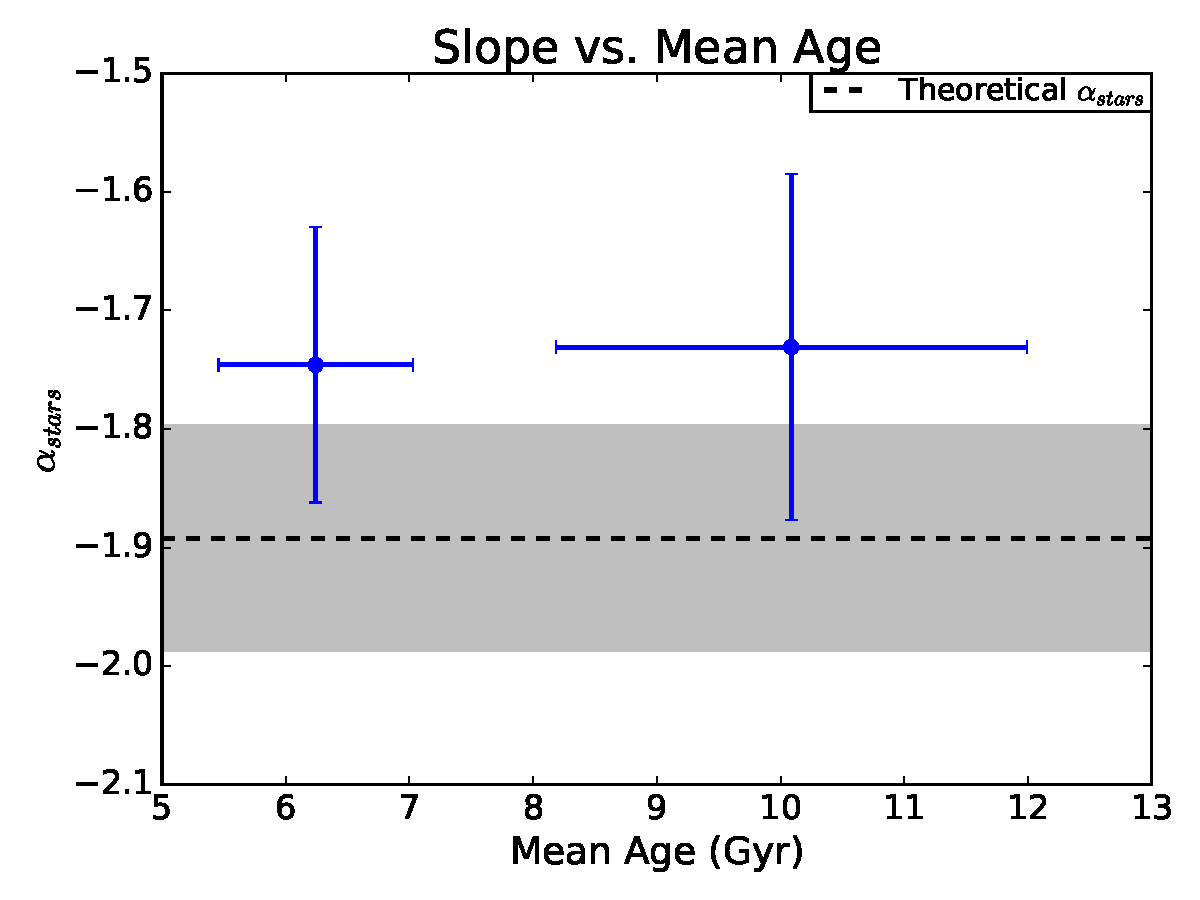
\includegraphics[width=.5\textwidth]{slopevmed.pdf}
\caption{The stacked slope ($\alpha_{stars}$) and mean age (blue points). The black dotted line represents the theoretical  $\alpha_{stars}$ within a gray confidence interval.}
\label{fig:svm}
\end{figure}

As a final representation, Figure \ref{fig:svm} shows the relationship between mean age and slope. Pillepich plotted the theoretical luminosity density to comoving distance for elliptical galaxies (\cite{Pillepich:2014}). As a frame of reference, we found the theoretical  $\alpha_{stars}$ for the same stellar envelope range we used in our stacked slopes (black dashed line with gray confidence interval).

We found that  $\alpha_{stars}$ is not dependent upon its formation time. It is also within $1\sigma$ of what we expect to get, according to Pillepich. 


\section{Conclusions and Future Work}

In conclusion, it is not necessary to remove bright objects (as long as we fit $\alpha_{stars}$ to the same physical range). We also found no correlation between accretion history and Star formation epoch, as determined by $\alpha_{stars}$. 

Our end goal is to find the relationship between $\alpha_{stars}$ and the Dark Matter Halo. Therefore, the next step is to use Weak Gravitational Lensing to get the total halo mass, and ultimately quantify the underlying total halo mass. 

This experiment can be varied. For example, we are only using one of HSC's six Wide Fields. We can expand to one of the other fields to have more galaxies and better statistics. Furthermore, we can use a different galaxy population. LRGs might contain too narrow of a Star Formation History range. We might want to try younger, more active, bright galaxies, such as CMASS. We can look at different bands. The \textit{i} band is deeper, and can go to fainter magnitudes. However, we expect better detection in \textit{g} because the difference between younger and older galaxies will be bluer. Most importantly, we should measure galaxies to larger apertures, so we have information that extends to the virial radius.

\clearpage
\bibliographystyle{apa}
\bibliography{LRG_DM}
\nocite{*}

\end{document}